%!TEX root = ../thesis.tex
\begin{savequote}[90mm]
	Scrum means ``Waterfall but we don't have time for analisys''\\
	Kanban means ``Scrum, but we don't have time for Sprint planning''\\
	Agile means ``We have no process but we do use Jira extensively''
	\qauthor{\href{https://twitter.com/mikeveerman}{@mikeveerman} on Twitter}
\end{savequote}

%Andando a vedere i contenuti di questa parte non mi soddisfano molto. Ce troppo scritto e poco di tecnico. Parla meglio un diagrama che 10 pagine di scritto.
%Di solito, per queste tipologie di lavori, consiglio di seguire un approccio top-down. Espongo un diagramma (di qualsiasi natura) che racconta l'intera soluzione e blochi che la compongono e poi vado a parlarti di alcuni di questi blochi e come si incastrano. 

\chapter{Projet implementation}
\label{chapter_5}

	This chapter is the core of this document and describes the way that this project has been implemented according to the planning described in Chapter 2.\\
	It is structured in four main sections that go over the main time periods presented in the Piano di lavoro document.\\
	Since the scope of the project was to create a demo environment to show the capabilities of Jira, Athonet has bough ten user licenses for Jira Software, ten for Service Desk and ten for Confluence.\\
	%todo inserire riferimento
	%https://confluence.atlassian.com/cloud/compare-atlassian-cloud-vs-server-744721664.html
	All these software have three installation options:
	\begin{itemize}
		\item Cloud: on their infrastructure
		\item Server: download and install on a local network
		\item Data Center: download and install for a large infrastructure
	\end{itemize}
	Because of Athonet's policies about storing their data in the cloud, they opted for an on premise Server installation.
	This kind of installment requires a one time payment for the software while other subsequent fees will be for the support.

	%todo togliere se non serve
	\newpage

\section{Learning phase}
	This phase corresponds to the first two weeks of the internship.
	As described in the work plan in this first period the main task was to understand what the tools are and what they can do.\\
	At first I have started to search information about Jira and Confluence on Google.
	%todo aggiungere riferimento a official documentation
	The first one I have started researching was Jira, and i found that the official documentation is very well organized.
	\begin{figure}[H]
		\centering
		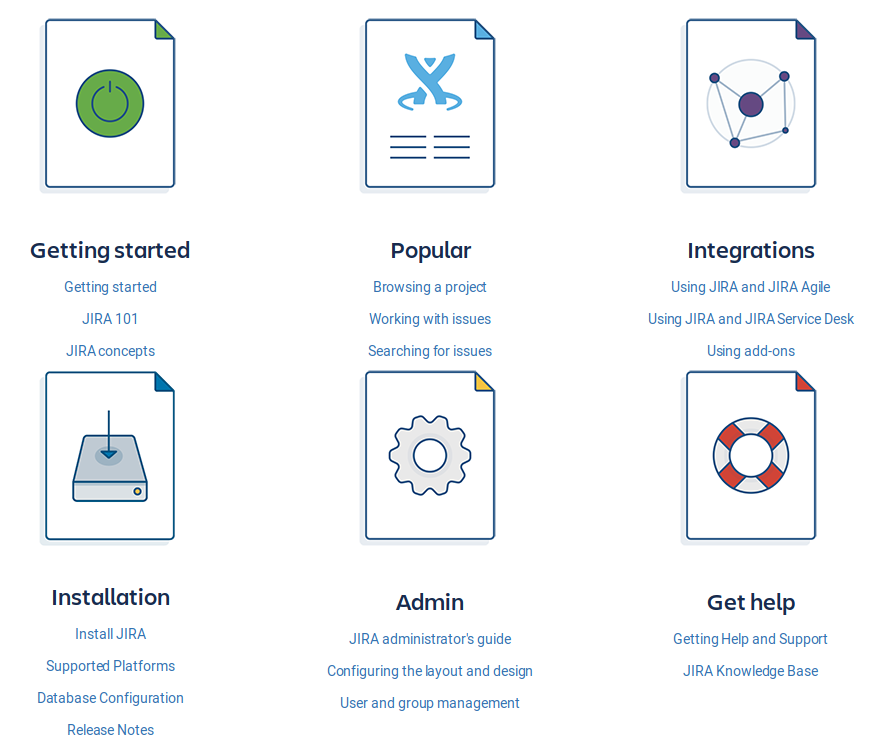
\includegraphics[width=1\textwidth]{resources/jira_documentation}\\
		\caption{Screenshot of the Jira Documentation homepage from the Atlassian Support website}
	\end{figure}
	It is very easy to navigate because it's versioned for each release, major and minor, of the software, plus it contains links to related pages, including Confluence's documentation and Atlassian's blog.
	%todo questa frase fa schifo
	%On Confluence's documentation, if there is a reference to Jira's, it links to the latter's documentation.	
	%todo aggiungere riferimento
	As said in ... both Jira and Confluence have a bug reporting and issue tracking section in their documentation.
	\begin{figure}[H]
		\centering
		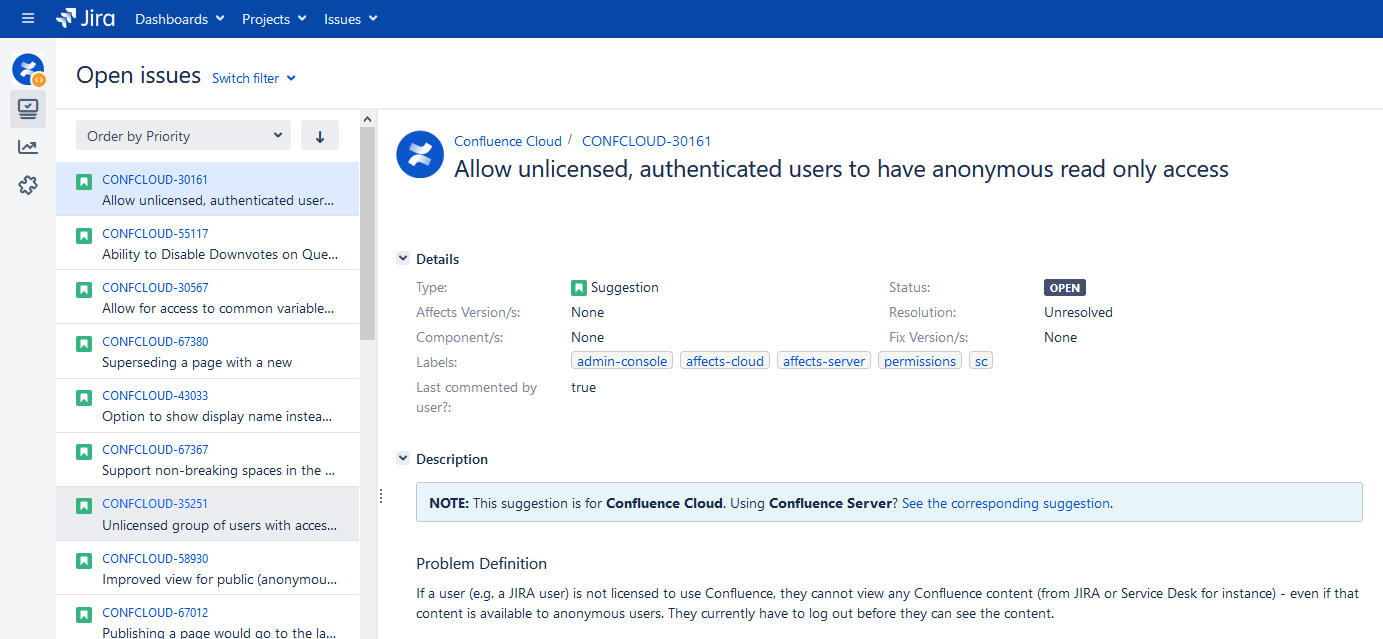
\includegraphics[width=1\textwidth]{resources/confluence_documentation_issues_1}\\
		\caption{The issues related with Jira and Confluence are handled by a dedicated Jira Cloud instance}
	\end{figure}
	If a web page in the documentation is related to an issue, this is showed at the end of the page with its status and a link to its dedicated section.\\
	%todo rivedere ripetizioni
	The Confluence and Jira documentation are both written and hosted using Confluence, showing how powerful can be this tool for handling a wiki for such a complex software that has a large userbase.\\
	Confluence's documentation is structured like Jira's, very easy to access and consult.	
	Another bonus is that it is public and free to read, despite the software is not.\\
	%todo cercare un'azienda che ha la documentazione privata
	%This may seem like an obvious choice for Atlassian, but not all vendors do it: RedHat for example let's you consult their documentation only if you log into the website.
	During the second half of the first week I went ahead and started configuring the environment.
	%todo spiegare acronimi
	%todo aggiungere a glossario centos
	In order to install the Atlassian tools I was given a CentOS VM with 512GB of storage and 32GB of RAM, connected to a special testing network environment for internship students.
	%todo aggiungere a glossario remmina
	To connect with the remote machine I used Remmina, a remote desktop client for Linux OSs.
	\begin{figure}[H]
		\centering
		
\includegraphics[width=.6\textwidth]{resources/centos_logo}\\
		\caption{The issues related with Jira and Confluence are handled by a dedicated Jira Cloud instance}
	\end{figure}
	
	
\section{Initial installation and configuration}	
	Since the documentation I found was very exhaustive, I decided to anticipate the installation phase so that I could have a more hands on approach.
	%todo rivedere frase
	I started to look on this more practical part from the second half of the second week and, although in the Gantt diagram it overlaps with the previous task, it's because it involves some study as well.\\
	%todo inserire citazione
	%https://confluence.atlassian.com/adminjiraserver/installing-jira-applications-on-linux-938846841.html
	As for the previous phase, I started by installing Jira following the official documentation.
	\begin{figure}[H]
		\centering
		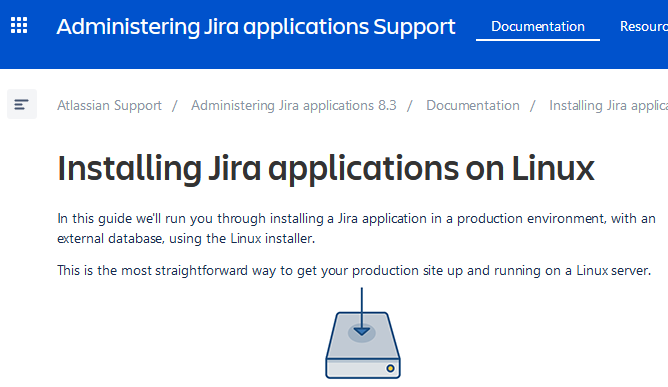
\includegraphics[width=1\textwidth]{resources/jira_installation}\\
		\caption{The issues related with Jira and Confluence are handled by a dedicated Jira Cloud instance}
	\end{figure}
	% todo aggiungere riferimento a paragrafo
	Jira needs a database in order to store all the information regarding projects, users, etc.
	For the first installation, used for testing purposes, the embedded H2 database was enough.
	%todo aggiungere a glossario h2 database 
	%todo aggiungere riferimento a documentazione
	%https://confluence.atlassian.com/jirakb/accessing-jira-s-h2-embedded-database-776818136.html
	It's important to note that the documentation says the H2 database is not suitable for production environments.
	%todo aggiungere immagine prima pagina di jira appena installato
	The first thing that I have done after the installation was getting acquainted with the interface and understanding how Jira's components interconnect with each other as I read in the documentation.\\
	To do this I have created some mock projects and filled them with issues; it's here that I understood the concept of Board in Jira.\\
	Boards and workflows are very tied in notions.
	Experimenting with workflows was one of the most important things to do, because these are fundamental in an issue tracking system's configuration and are strictly connected to Boards.
	
	% todo inserire immagine di board
	
	After understanding the fundamentals of this software and getting to know it's basic features, I went ahead and installed Portfolio.
	%todo aggiungere riferimento
	This plugin, as told in ... helps visualizing the issues on a roadmap, which was one of the most important requirements.\\
	%todo aggiungere riferimento a requisito
	Installing Portfolio was easy, I just followed the instructions on the documentation to download the latest version of the plugin and embed it to Jira.
	
	%todo inserire immagine di portfolio
	
	After installing this plugin and creating plans for my mock up projects, I have chosen to install Service Desk, to complete the configuration of my Jira instance.
	%todo inserire \cite a website
	As earlier I have followed the documentation on the website.
	%todo aggiungere riferimento
	%todo aggiungere portal a glossario
	As described in ... this piece of software is used to communicate with the clients and having a portal from which a client can find information and request assistance with a product.
	The first thing I tested after installing this software was creating a help center and see from the point of view of a client how this can be able to open an issue and what type of issues he may have access to.
	
	%todo inserire immagine Service Desk
	
	%TODO CHE SENSO HA QUESTA FRASE
	After I became familiar with Jira, I have installed Confluence, and like for the other software, I have used it's embedded database.
	Both software run on the same system, and their services are offered on port 8080 and 8090 respectively for Jira and Confluence.\\
	During installation I connected them together and tested the environment by creating a knowledge base for a Service Desk project and a documentation space for a Software project.\\
	Confluence was easier to get familiar with, so after creating some mock spaces related to the projects that were in Jira at the time, I moved on.
	%todo on either one of the instances
	To ease the integration between these tools, Atlassian allows to have a single users table stored on either Jira or Confluence.\\
	This was shown during the installation of Confluence as an option to link it with Jira's instance was presented, I inserted the administrative credentials and told it to use Jira's users.
	%todo aggiungere a glossario tomcat (con immagine) e webserver
	%todo aggiungere riferimento a http://tomcat.apache.org/
	Jira and Confluence both use an Apache Tomcat web server.
	To run them both on the same domain I had issues regarding the login.
	Cookies for the users are stored for allowing them to access without inserting the password each time, but they didn't work correctly because the users were automatically logged out after some minutes.
	This was because, when running on the same domain, even if on different ports, cookies from Jira and Confluence go in conflict.\\
	%todo aggiungere riferimento
	%https://confluence.atlassian.com/jirakb/how-to-change-the-jira-application-context-path-225119408.html
	While seeking the Internet for answers, I found that many people new to these software gt into the same situation.
	%todo inserire a glossario context path con riferimento da
	%https://www.eclipse.org/jetty/documentation/9.4.x/configuring-contexts.html
	To solve this issue all is necessary is to change the context path of the software's server.xml file that contains the configuration of the web-server.
	An example of changing the context path for this project is:
	\begin{center}
		\texttt{http://yourdomain.com:8080}
	\end{center}
	becomes:
	\begin{center}
		\texttt{http://yourdomain.com:8080/jira}
	\end{center}
	For Confluence, where the default port is 8090, the context path will become:
	\begin{center}
		\texttt{http://yourdomain.com:8090/confluence}
	\end{center}
	At this point there was a change in the requirements that were given to me by the tutor.
	Contrary to what he said in the beginning, the IT department opted to use GitLab instead of BitBucket because the developers know it better and there is no billing for their usage tier.	
	%todo togliere?
	So it's free.
	
	%todo mettere immagine logo gitlab
	
	This meant that there would be one less tool that needed to be installed, but I had to understand how to link Jira's functionalities to those offered by GitLab.\\
	Connecting these tools together means that a developer can interact with Jira's issues in a project by typing it's ID in the messages that he uses for commits, comments, merge requests and so on.
	Fortunately GitLab's documentation had a dedicated page with instruction examples and a guide that allowed me to configure both tools.\\
	%todo citare
	%https://docs.gitlab.com/ee/user/project/integrations/jira.html
	This functionality allows GitLab to interact with Jira's default workflows, which sometimes are too simple for some software projects.\\
	Since the license for GitLab's hosted version is not Premium (or Silver for the online one) there is no interaction the other way around, from Jira to the repository.
	%todo citare
	%https://docs.gitlab.com/ee/integration/jira_development_panel.html
	Because these tools are not strictly related, there is no 1:1 project mapping from GitLab to Jira, a commit message in the repository may reference multiple Jira issues from different projects, so it's the programmer's discretion to comment wisely.
	%todo aggiungere riferimento
	Later ... I will talk about installing a plugin that allows these tools to be better connected.\\
	After understanding the potentiality of this connection I went on and set up a small demo that touched all the things that I have covered in the first two weeks of the internship.
	Since my tutor wasn't available for a few days so I took the liberty to customize the environment by changing the colors and logos in the interface, putting Athonet's.
	
	% todo inserire immagine di interfaccia customizzata
	
	When he came back during the meeting I have taken with him, he said that he liked the work I have done and that it was time for more elaborate mock projects in order to present the tools' functionalities to other company figures.\\
	After that I have deleted the mock projects from Jira and the related spaces in Confluence to ask the IT department for a snapshot of the VM I was working on.\\	
	%todo correggere se da altre parti c'è scritto milestone
	This allowed me to have a baseline, a deliverable that I was able to use as a secure point in time in which I could go back if anything after went wrong.
	
\section{First realistic mock projects and feedback}
	The fourth week of the internship I was ready to implement more realistic projects in Jira, connecting them to Confluence providing them with documentation and creating a link with GitLab.
	The objective was to finalize the working demo that could be shown to various members of Athonet for them to understand how these software can be used in their departments.\\
	In Jira I have created the projects EPC and Dashboard, both Software, while in Confluence I have created the spaces EPC Documentation and Dashboard Documentation.
	Also in Jira I have created an Athonet Internal Wiki project, to show how Service Desk could be useful for sharing internal documents between employees.\\
	For the first project I have implemented a more articulate workflow that resembles the realistic evolution of an issue inside the company and customized the menus that allow the creation of an issue.
	
	%todo inserire immagine workflow
	
	Later these will be revised because in this stage I was not given the information about what an issue requires to have in Athonet's case.\\	
	As I continued working on the mock projects and creating issues, I noted down all the most important customization that an administrative user can use to set up the software, not only for Athonet's specific purposes but in general.\\	
	To make the project more realistic I have created three user groups, besides the default ones, to which I have assigned three users each:
	\begin{itemize}
		\item Management
		\item Verification
		\item Developers
	\end{itemize}
	%todo va bene ;?
	Every group had various permissions; this allowed me to demonstrate how basic security rules work in these tools.\\
	After telling the progress I have made to the tutor, he was able to set me a meeting with himself and the verification and developer managers.
	%todo aggiungere riferimento
	I then prepared some slides to explain some of the nomenclature in Jira, as explained in ..., and the various things that I have implemented.\\
	The core of this meeting was a discussion between the managers focused on understanding how their ongoing projects could be implemented in such a way that the employees would not be forced into using a strict Agile methodology, but to accommodate and let them understand how these tools work without creating chaos.\\
	There was a discussion on how applying a strict Agile methodology could impact their time division.
	Agile provides sprints that by definition last two weeks.
	These produce deliverables that bring added value to the project.
	Athonet's line of work though is focused on adding value to the product upon new releases that are scheduled differently by their purpose:
	\begin{itemize}
		\item Bug fix
		\item Minor release (for patching issues with the code or to improve performance)
		\item Major release (for new features)
	\end{itemize}
	Sprints would disrupt the routines of the developer team, the verification team and of management.
	In this case it would not be the tool that adapt to the company but vice versa the company would need to change in order to use the tool and would be counterproductive.\\
	The developer manager stated that he wanted a way to measure productivity, so I showed him the reports section that is present for all kind of Jira projects.
	
	%todo inserire immagine reports
	
	Since he was not keen on the strict Agile interface with the backlog composed only by the issues that were meant to be completed in a two week period, he wanted me to show how the kanban board looked like.
	
	%todo inserire immangine board
	
	He said that it would be better for the company's way of work since developers could program their work based on what has to be completed for the next release, so for a longer period of time.\\	
	This implied there would be a more particular workflow that had to be implemented and the managers were happy to see that it could be easily done, as for customizing the issue creation and modification menu.\\
	They were also happy about the Internal wiki project because it suggested there could be one single tool for both internal documentation regarding clients and general notes for employees (like for example a guide on how to install Docker without loosing internet connectivity).\\	
	After this meeting, I was put on standby because of the internal discussions that had to be done in order for the managers to understand how to adapt the workflow they had in Redmine for Jira and how to include Confluence in the mix.
	This was not considered when writing the piano di lavoro document, but to carry on with the work I decided to start writing the documentation about installing and configuring the software, aimed for the system administrators in the IT department.
	In the sixth week I showed it to the tutor and, after his approval, I started working on the user guide, which was written in the wiki Confluence space.
	In order for the users to understand how to use the tools, they had to start using them.
	
	%todo ci sta veramente come parte? alla fine ok ho fatto ma non verrà mai usata come cosa
%	There was an issue I noticed that would not allow unlicensed users, to enter the wiki.
	
	%todo project e product quoted 
	Later on, a new meeting was scheduled with the product owner, who wanted to understand better Portfolio and how the concept of product matches the project denomination in Jira.
	
	%todo citare
	%https://harbott.com/whats-the-difference-between-a-product-and-a-project-aaacfc983340
	Project and product sound similar and the two concepts are often confused with each other.
	A project is a temporary endeavour, with a clear definition of what needs to be delivered and by when, it has a beginning and end date.
	A product is designed to continually create value for customers by solving their problems.\\
	For the product owner, one of the most important things was to see how releases are mapped inside the software, since Redmine did not offer such an intuitive interface and did not allow to see them on a timeline and applying custom filters.
	I showed him the progress I have made and he approved it, also he said that he wanted the credentials to start using it and see how to map the ongoing projects in Redmine to new ones in Jira or how to migrate them.\\
	After using it for a couple of days and talking with the other managers, I was given a feedback on how Athonet would use these tools.
	Since they were not sure letting users access Service Desk directly, an employee would create an issue that would represent the customer request through service desk.
	The customer request could be a new feature, a bug report, require support, etc.
	This would then be picked up by a team that would bring it inside a Business type of project by creating a linked issue.
	This project would have a particular workflow and contains the more high lever tasks like documentation, meeting notes, feature statuses, etc.
	These shared notes and documents would be stored in Confluence, where there would be links to them.\\
	After they have been approved for production another team would create a linked issue inside the software project.
	This would most likely be divided in many sub-issues by the team leader and these would be visible by the developers.
	Each developer could then pick an issue to work on and handle it as he wants by, for example, dividing it in smaller sub-issues.\\
	The next week I had another meeting with more company figures: a senior developer, the business strategy manage, the managers that I have talked to in previous meetings, the CTO and my tutor.
	As in the other meetings I have explained the various software that I have installed, the purpose for each one of them and the evolution of an issue.\\	
	Again, to have a milestone, I have requested a snapshot of the machine by the IT department.
	Even with the requirements changes I was on schedule with the Gantt diagram and the other planning.

\section{Transitioning into Production and final feedback}

	Although in the first planning this was a longer period of time, this last phase was shortened to a week.
	%todo subordinates va bene?
	This was due because of the many internal discussions that took place for the software to be approved and for the various managers of the departments to figure out how to introduce it to their subordinates.\\
	After the last meeting described in the previous paragraph, I have created new users for the managers that participated and gave them the credentials so that they could see the interface and interact with the mock projects that remained there.\\
	The tutor had credentials as well and he was very enthusiast of how the demo performed and the potentials of the software, although this had to be well understood by the other managers and members of the company as well.\\
	Although the last snapshot of the VM that was made contained a working infrastructure ready to be moved in a production environment, the IT department opted to wait until they understood how to properly secure the server that was going to host it.
	%todo aggiungere VPN a glossario
	The most important part would be creating a secure VPN tunnel that would allow outside employees that are working from other locations to connect as they would be inside the building.
	This method must ensure thought that there would be no possibility for any other to get, or even hack, inside the company's network and access their products' source code.
	Besides this, the other managers where very glad to hear that the tools have been approved and where happy about the demonstration.\\
	%todo rivedere bene
	Because this, I was not able to migrate any data from Redmine's instance to Jira, since I was not granted permission to access the company's private data about the source code and even if the migration would have been successful it would have not been used when Jira and Confluence were moved into production.
	The CTO of the company and PriMo's product owner were interested in the possibility of using a real time roadmap to keep track of the work done while not going as in deep as seeing the tasks assigned to each developer.	
	
\section{How are these tools being used}
	
	%I prefer to use more soft and vague statements, like "Even if Athonet does not go for a pure agile development's model, the tools can still help to improve the organization of their work. In fact, the tools fits their current needs, which reflect an hybrid model between Scrum and Kanban: Scrumban"
	
	Athonet does not want to pursue being an Agile software developing company in the near future, but it wants the tools that allow to organize their projects such that if one day their strategy varies, then the software would follow along.
	What they really want adopt now is a hybrid between Scrum and Kanban: Scrumban.\\	
	As in Kanban visualizing workflow, limiting work in process (WIP), and measuring productivity are prioritized.	
	Scrumban removes the practice of limiting WIP by time (i.e. velocity and Sprint boundary) and replaces it by limiting WIP for each stage.
	It's based on having a continuous flow of work, which is what Athonet has for their products.\\	
	%todo citare
	%https://www.atlassian.com/agile/kanban/kanplan
%	In Jira this aproach is called kanplan and it's well doucumented on.
	